%
% File naaclhlt2010.tex
%
% Contact: nasmith@cs.cmu.edu

\documentclass[11pt,letterpaper]{article}
\usepackage{naaclhlt2010}
\usepackage{times}
\usepackage{latexsym}
\usepackage{amsmath}
\usepackage{hyperref}
\usepackage{graphicx}
\DeclareMathOperator*{\argmax}{arg\,max}
\setlength\titlebox{6.5cm}    % Expanding the titlebox
\usepackage{tabularx}

\newcolumntype{b}{>{\centering}X}
\newcolumntype{s}{>{\hsize=.2\hsize}X}

\title{A Network-Assisted Approach to Predicting Passing Distributions}

\author{Angelica Perez\\
	Stanford University \\
  {\tt pereza77@stanford.edu}
  \And
  Jade Huang\\
  Stanford University \\
  {\tt jayebird@stanford.edu}}

\date{}
\pagenumbering{arabic}
\begin{document}
\maketitle
\begin{abstract}
% What is it that you are trying to solve/achieve and why does it matter?
We introduce an approach of using a linear regression model plus stochastic gradient descent to predict the passing distribution of a soccer team based on data from the UEFA Champions League. Features are derived from player-specific statistics, team-specific history, and network measures while weights are learned to predict the number of passes between each pair of players on a team. Our linear regression model with features and SGD achieved a 25.27\% improvement in the average loss from our baseline model of only average past passing networks.
\end{abstract}

\section{Introduction}
The passing network of a team can reveal much about game strategy--who the key player or key players are, whether a team had a hard time against its opponent and focused mainly on defense or if it was completely dominating its opponent and was rocking the offense. Furthermore, the passing network changes based on the opposing team--team A will play differently when faced with inferior team B than when faced with superior team C. 

Given the history of passing networks of team A and another team B, predicting the passing networks of both teams ahead of time has a number of implications. We can uncover the different patterns of how a team plays another team of a certain difficulty. We can predict the layout of future games, winning more bets, and perhaps giving teams a leg up on their competitors by giving them clues on how their competitor may play based on their playing history.

%Thus our objective is as follow: given a team A's past passing distributions, a team B's past passing distributions, the average lineup of team A, and the average lineup of team B, the goal is to predict the edges between players for both team A and team B when team A and team B face each other in a match.

%Due to the observation that lineups do not change dramatically for a team between matches, we randomly choose a lineup used by a team during the group stage and hold it as constant as we seek to predict the edges between players.

\section{Problem}
% TODO
Given a match between two teams $A$ and $B$, each of their starting lineups, and each team's passing history comprised of $t$ past passing distributions $PD^{(A)} = \{pd^{(A)}_1, pd^{(A)}_2,…,pd^{(A)}_t\}$ and $PD^{(B)} = \{pd^{(B)}_1, pd^{(B)}_2,…,pd^{(B)}_t\}$ along with additional team and player statistical data, our model seeks to predict new passing networks $pd^{(A)}_{t+1}$ and $pd^{(B)}_{t+1}$ for each team.  We use a linear regression model to learn feature weights using stochastic gradient descent that are then used to predict the edge weight, or number of passes, between each pair of nodes, or teammates, in match $t+1$. 

The features are comprised of a variety of UEFA data and attempt to encapsulate the necessary team and player characteristics to predict edge weights, such as team rankings, average passes between a pair of players, and average betweenness of  a player. We carefully choose features that accurately describe a pair of player's historical relationship on the field, the typical involvement of an individual player amongst his team, and, equally as important, a team's strategy and passing history, including how a team's style of play (i.e. heavy midfield or light offense) may change against a specific opposing team.  

\section{Related Work}
% How does your project relate to previous work. Please give a short summary on each paper you cite and include how it is relevant.

\cite{Pena:12} uncover how players perform on a team by analyzing centrality measures such as closeness, betweenness, PageRank, and clustering. The authors found that through betweenness, one can uncover which players are more involved. If the network is very complete with most edges between most or all players, one can say the team is very well-connected. \cite{Grund:12} expands upon \cite{Pena:12} with two hypotheses that he confirms in his paper: 1. increased interaction intensity leads to increased team performance and 2. increased centralization of interaction in teams leads to decreased team performance. Using the mean degree (volume of play), variance degree (diversity of play), and harmonic mean of the mean and variance degree of the player passing network, \cite{Cintia:15} achieved 53\% accuracy in predicting match outcomes.

Building upon \cite{Pena:12}, centrality measures, especially betweenness centrality, can be used as features in predicting edges between players. A player with a higher centrality measure perhaps will receive more passes on average.  Features used by \cite{Cintia:15} and \cite{Grund:12} such as mean degree, variance degree, interaction intensity, centralization of interaction are indicative of team-specific patterns and can be used in our model when predicting edges. 

Due to limitation of data from FIFA, \cite{Pena:12} computed passing networks by dividing the number of passes by the total number of plays played by each team, lacking a per-game analysis which could be indicative since a team most likely does not play the same way with all opponents. Similarly, \cite{Cintia:15} and \cite{Grund:12} fail to acknowledge how team dynamics will perform in relation to the dynamics of an opponent. \cite{Grund:12} defines the most centralized network as the one where most interactions involve the same two individuals. However, such a definition can be further expanded to include cases such as where all members of a team pass to one central player equally.

\section{Model}

% This is where you give a detailed description of your primary contribution. It is especially important that this part be clear and well written so that we can fully understand what you did.

\subsection{Baseline}

For a baseline model, the average of past passing networks during the group stage is used to predict the passing networks during the round of 16 stage. Thus, during training, for every player to player combination in each team for which there exists a pass, the total number of passes over six games is calculated during the group stage and averaged over the number of games. 

The average values calculated during training are used to predict the number of passes for each team in each game in the round of 16 of the 2014-15 season. For example, if in team X, player 1 passed to player 9 an average of five times during the group stage, this baseline model would predict that player 1 would pass to player 9 five times when playing some team in the round of 16.

This is a naive baseline that does not take into account the specific opponent during each of the past games during the group stage, but merely generalizes, ignoring any idiosyncrasies which may arise when facing a higher ranked or lower ranked opponent. 

\section{Algorithm}

To build upon the baseline, a linear regression model was constructed to include features that are indicative of the amount of passes between two players and which would learn weights which would correspond how descriptive a feature is in relation to the amount of passes between two players.

\subsection{Features}
With guidance from Tim Althoff, we postulated the following are key ingredients leading to how often two certain players pass:

\begin{itemize}
\item \textbf{Average number of past passes between two players}, a continuous value that is pre-computed before the process of training and learning weights and averaged over the group stage. As with the baseline, the average of all passes between two players for each player for each team over all "past" games, where the notion of past is experimented with later on, is taken.
\item \textbf{Whether two players are of the same position}, firing $1$ if the condition is true and $0$ otherwise. The motivation for this feature is that based on analyzing the data, certain positions pass to each other very often, such as from defender to midfielder, while others never pass to each other, such as goalkeeper to goalkeeper. Please see \ref{fig:barGraph} for a bar graph showing the number of passes made between each position in a game between APOEL FC and Paris Saint-Germain. Similarly, we also have a feature for whether two players are of different positions. 

\begin{figure}
\caption{Number of passes made between each position in a game between APOEL FC and Paris Saint-Germain.}
\centering
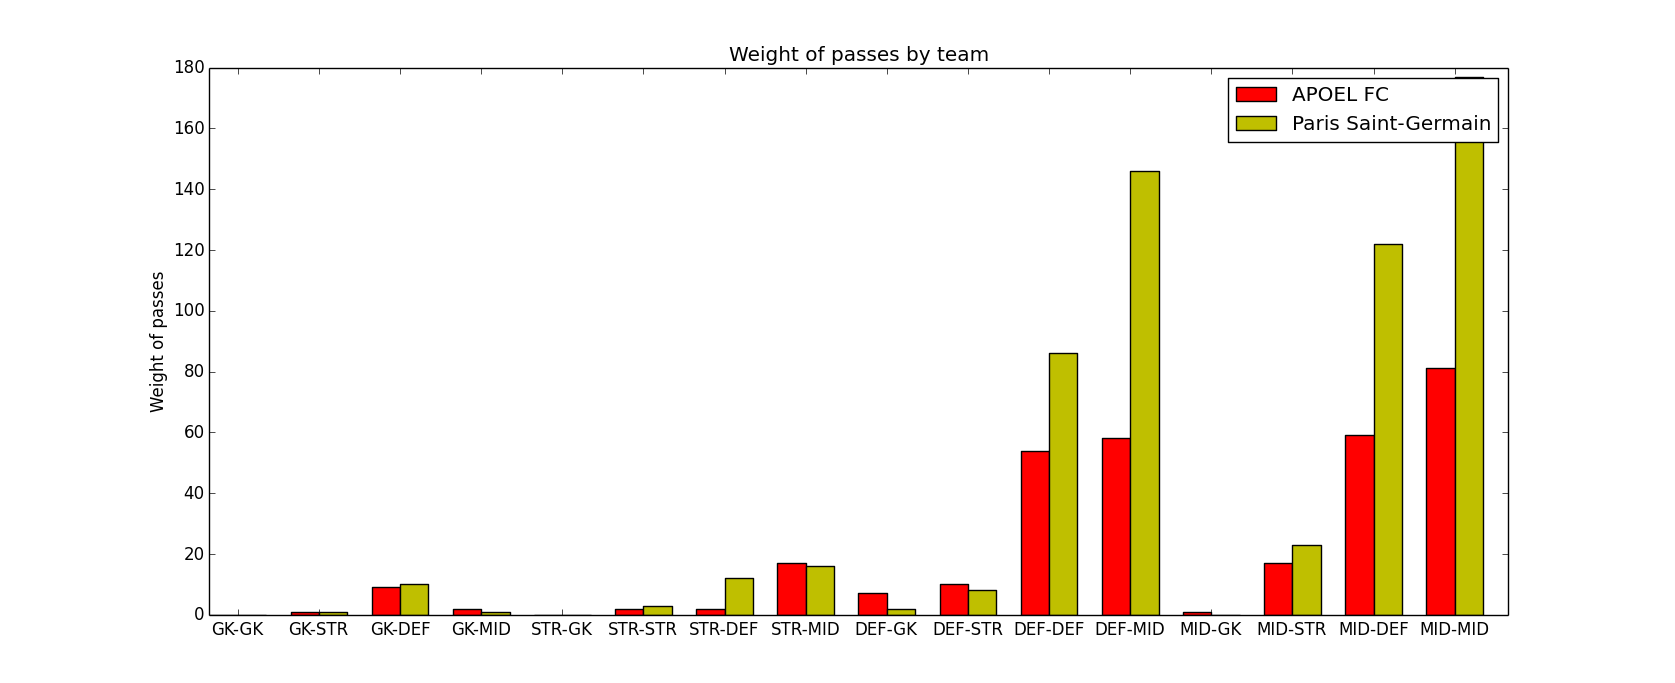
\includegraphics[scale=0.20]{APOEL_FC-Paris_Saint-Germain.png}
\label{fig:barGraph}
\end{figure}

\item \textbf{Whether team A's rank is higher than team B's rank}, firing $1$ if true and $0$ otherwise. The motivation is that perhaps players may pass more or less depending on whether the opponent team is ranked higher or lower. 
\item \textbf{Whether team A has won against a "similar" team as team B in the past}, firing $1$ if true and $0$ otherwise. In every subsequent stage, teams play teams that they haven't played in previous stages--thus there is no previously existing data stored for team combinations at testing time. Thus, it may be helpful to find a team C that is similar to a team B in team A's play history and use the outcome of that match in determining if team A has a good chance of winning against team B.
\item \textbf{Whether team A's average pass completion rate is higher than team B's pass completion rate}, firing $1$ if true and $0$ otherwise. The average is taken of pass completion rates across past games ignoring specific opponents. Similarly we also have features for whether team A's average passes attempted and average passes failed are higher than team B's pass completion rate. In analyzing the data, a trend was observed where 63.5\% of the time the team with a higher pass completion rate and was also the team that lost the match. Also, 62.5\% of the time the team with a higher number of passes attempted was also the team that lost the match.    
\item \textbf{Average number of passes between two positions on a team}, a continuous value. The motivation is that perhaps on a team, two given positions generally pass to each other some similar amount across all games.
\item \textbf{The average betweenness centrality of both players} respectively averaged over games during the group stage. As mentioned in related work, betweenness centrality can indicate the importance of a player, of how often the player is a cog in between passes.
\item \textbf{Average percentage of passes completed for two specific players} averaged over percentage of passes completed during the group stage, a continuous value. The intuition is perhaps it is more likely for two players to pass if their percentage of passes completed is higher.
\end{itemize}

\subsection{Evaluation}

We utilized the squared loss to capture the accuracy of a prediction of number of passes between two players in comparison to the actual number of passes between two players. The score $\phi(x) \cdot \mathbf{w}$ is considered the prediction while $y$ represents the actual number of passes.

\begin{align*}
Loss_{squared} &= ({\tt predicted} - {\tt actual})^2 \\
&= (\phi(x) \cdot \mathbf{w} - y)^2
\end{align*}

To evaluate our model as a whole, we took the average of the loss over all passes between players. In the below equation, $T$ represents the total number of passes between players over all teams and games during the round of 16 stage.

\begin{align}
Loss_{model} = \frac{1}{T} \sum_{i = 0}^{i = T} (\phi(x) \cdot \mathbf{w} - y)^2
\end{align}

\subsection{Learning Weights}
Our linear regression model learns weights using stochastic gradient descent. The objective is to minimize our squared loss, thus with every new training example, i.e. number of passes between two players, we update our weights with the following equation:

\begin{align*}
w &\leftarrow w - \eta \nabla_w Loss \\
w &\leftarrow w - \eta 2(\phi(x) \cdot \mathbf{w} - y)\phi(x)
\end{align*}

where $\eta$ is the step size controlling the rate of descent.

\subsection{Data}
Data used includes team passing distributions, tactical lineups, and squad lists provided by the UEFA Champions League press kits for the Group, Round of 16, Quarter-finals, and Semifinal stages of the \href{http://www.uefa.org/mediaservices/presskits/uefachampionsleague/season=2015/index.html}{2014-15 season}. Team rankings were taken from the \href{http://www.uefa.com/memberassociations/uefarankings/club/season=2015/index.html}{UEFA rankings for club competitions} for the 2013-14 season. We implemented Python and bash scripts to parse this set information for a total of 124 games for 32 teams, with a total of $26,358$ passes between $3,428$ players over $248$ networks with an average of $13.8223$ players per team and $106.2823$ passes per team.

For each team for each game in each stage, passing distributions included number of passes completed between all players as well as the total number of passes completed and attempted while squad lists included player names and positions.

\section{Results}

% How do you evaluate your solution to whatever empirical, algorithmic or theoretical question you have addressed and what do these evaluation methods tell you about your solution? It is not so important how well your method performs but rather how interesting and clever your experiments and analysis are.

% We are interested in seeing a clear and conclusive set of experiments which successfully evaluate the problem you set out to solve. Make sure to interpret the results and talk about what we can conclude and learn from your evaluations. Even if you have a theoretical project you should have something here to demonstrate the validity or value of your project (for example, proofs or runtime analysis).


\subsection{Baseline}
The baseline model has an average loss of $15.00$, which was calculated by summing up the individual loss for each player to player pass and dividing by the total number of passes during the round of 16 stage. 

For the predicted number of passes to differ from the actual number of passes by $15.00$ on average can be explained by the generalization made when averaging over all past passes. In addition, the games played during the Round of 16 have teams playing other teams that they did not play during the Group stage. Thus, the baseline is utilizing data that while generalizes how much players will pass to each other on average, fails to capture any changes in style a team may implement in the face of different opponents. 

\subsection{Linear Regression Model}
\subsubsection{Using shared model weights}
%We first experimented with using one set of weights for the model, disregarding differences in teams.

%No matter how many iterations are run through the six matchdays in order of increasing matchday in the group stage, the following results arise,

%\begin{tabular} {|c|c|}
%\hline Feature Added & Avg. Loss \\ \hline
%Average Passing Networks & 14.3420 \\ \hline
%+ Same Position & 13.6145 \\ \hline
%+ Different Position & 11.7954 \\ \hline
%+ Higher Rank & 11.8618 \\ \hline
%+ Won Against Similar Team & 12.0889 \\ \hline
%+ Avg. Passes Betw. Positions & 12.1446 \\ \hline
%+ Higher Avg. Pass Volume & 12.2467 \\ \hline
%+ Higher Pass Completion \% & 12.5603 \\ \hline
%\end{tabular} 

%At first, we were perplexed that even if we ran two iterations or ten iterations we still arrived at the same weights. The weights were being updated with every example, but despite initializing at zero or at the final weight, the weights settled into the exact same value. It appeared to be a bad case of overfitting.

%As an experiment, we shuffled the order of matchdays and found that the weights varied with each iteration, but upon test time, increasing the number of iterations didn't necessarily mean that the average loss decreased during testing time. Realistically, it does not make sense to shuffle the matchdays, as the matchdays occur in chronological order and a sort of history is accumulated.

%For a more realistic experiment, we shuffled the order of games in each matchday each iteration. As with the experiment of shuffling the order of matchdays, it became evident that resulting weight is dependent on the order of the games and when using even just one feature, the resulting average loss from the resulting weight can vary from $14.512204$ to $18.511490$. By doing away with overfitting, we were left with a large amount of variance. Again, increasing the number of iterations during training time didn't necessarily mean a lower average loss during testing time.

%While overall adding in additional features with a linear regression model that learned weights decreased the average loss from the baseline by 21.36\% at best, we experienced issues of overfitting when iterating through the data in a chronological order and, on the other spectrum, issues of variance when shuffling the data during training time.

% Added by AP
Experimenting with various subsets of features proved to be very interesting.  The features that computed average passes between two players, difference in team rank, whether two players are the same or different position lowered the loss consistently no matter which additional features were added to their sets.  Intuitively, these three features have a lot to do with how many times two players will pass to each other.  The average passes between two players is arguably the most indicative feature since that is the precise value we are attempting to predict.  Difference in team rank is a good indicator of which team will possess the ball for the majority of the game and by how much, so for a team that is far better than their opponent, the feature accurately raises edge weights across the board for the entire team. Examining if two players are in the same position also accurately raises edge weights as it is more frequent for two such players to pass to each other due to sheer proximity on the field.


\begin {table}
\begin{center}

\begin{tabularx}{\columnwidth}{|X|c|}
\hline \bf{Feature Set} & $\mathbf{\Delta Loss}$ \\ \hline
Average Passing Networks & 0.917 \\ \hline
Same Position & 0.069 \\ \hline
Difference in Team Rank & 0.506 \\ \hline
Mean Degree & 3.078 \\ \hline
Betweenness of Receiving Player & 5.774 \\ \hline
Average Pass Completion \% of Passing Player & 0.096 \\ \hline
\end{tabularx} 

\caption {Best-performing feature set in Shared Weights Model. The average loss for the set is 11.21. The losses listed are the increase in average loss when the specified feature is removed from the set.}
\end{center}
\end {table}

The average pass completion percentage for the passing player in a pair of teammates slightly reduced the loss consistently as well. It makes sense that a higher completion percentage will increase a player's out-edges.

We observed interesting outcomes during the use of combinations of three features: average betweenness of the passing player, average betweenness of the receiving player, and the mean degree of a team per match. Contrary to our hypothesis,  average betweenness of the passing player performed better 

\begin{figure}[h]
\caption{Predicted passing distribution for Juventus during the Round of 16 when playing against Borussia Dortmund.}
\centering
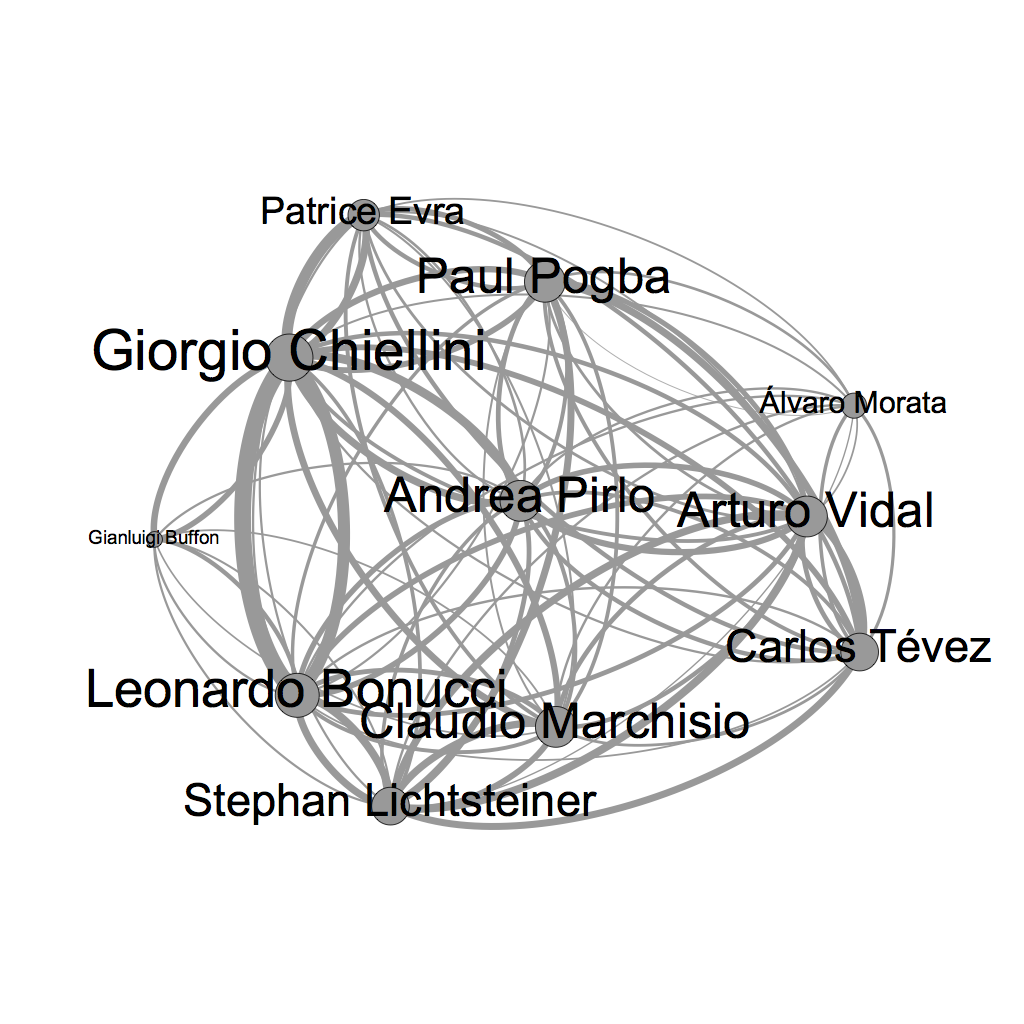
\includegraphics[scale=0.20]{2014408-Juventus.png}
\label{fig:Juventus-pred}
\end{figure}

\begin{figure}[h]
\caption{Actual passing distribution for Juventus during the Round of 16 when playing against Borussia Dortmund.}
\centering
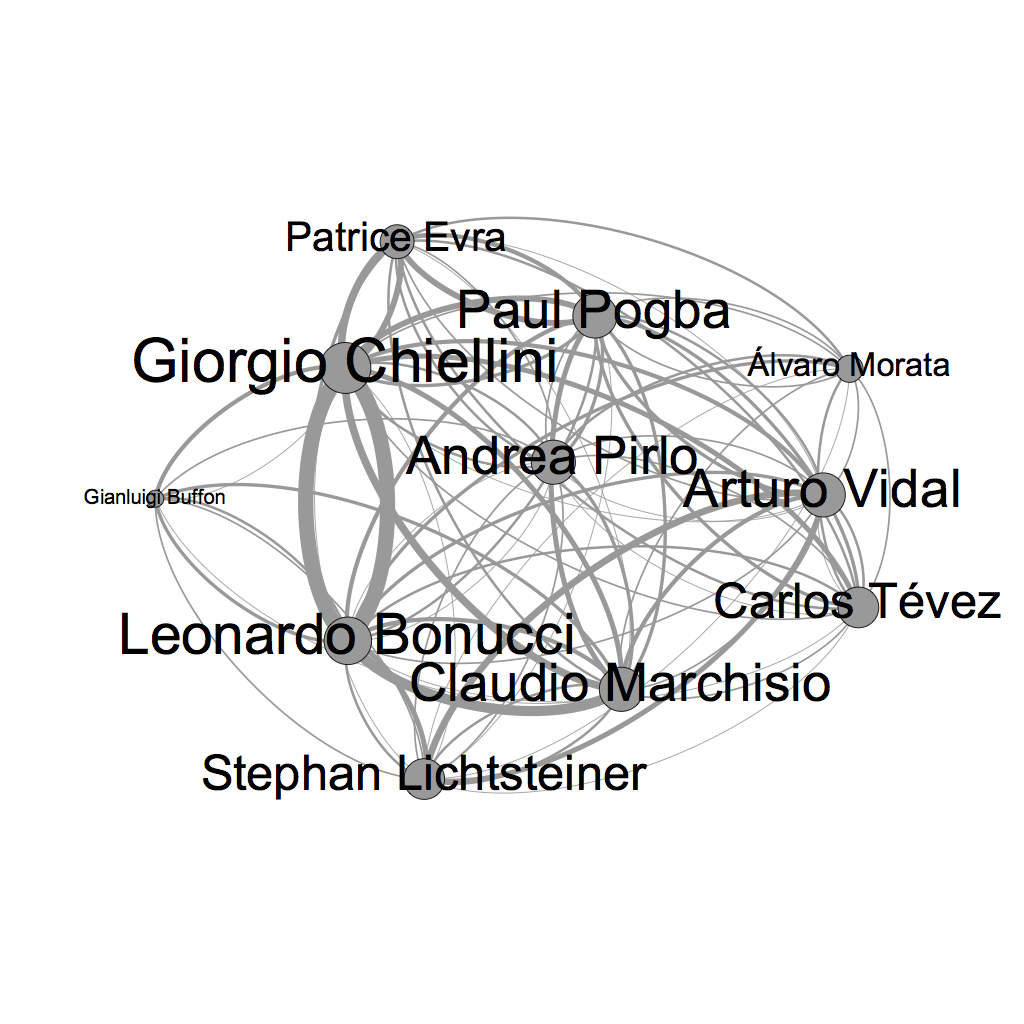
\includegraphics[scale=0.20]{2014408-Juventus-actual.png}
\label{fig:Juventus-actual}
\end{figure}

than average betweenness of the receiving player and the use of both features in the same set performed even worse than using only one of them.  We expected the combination of both to produce the least amount of loss since both players' centrality in the lineup seems important to the frequency of the two connecting.

Additionally, we found that average betweenness of the passing player consistently reduces loss when used in a feature set that does not include the other two features, but using both average betweenness of the receiving player and mean degree in a feature set without average betweenness of the passing player has an even greater positive impact on the loss. We hypothesized that mean degree would have less of an impact on the magnitude of edge weights since it does not really capture the relationship between two players or the team's strategy against a specific opponent. Moreover, other features in our experiments, such as difference in team rank and whether a team has won against a similar opponent in the past, seem to be better indicators of the number of passes an entire team will make against a certain opponent.  Yet, our best-performing set of features includes mean degree, which only performs well with betweenness centrality of the receiving player.

Figures \ref{fig:Juventus-pred} and \ref{fig:Juventus-actual} above depict the predicted and actual passing distributions of the team Juventus against Borussia Dortmund during the Round of 16 stage. Our predicted network generally has more edges than the actual network, as it is more likely to predict a real value that is non-zero than zero due to the nature of our scoring function. What is exciting is that our predicted network was able to capture the concentrated movement along the defensive line of Evra, Chiellini, and Bonucci. This defensive line is not always so concentrated, as can be seen in a game against Malmo FF during the group stage (figure \ref{fig:Juventus-group} in the Appendix), where the passing concentration is more heavily weighted in the midfield and more spread out, thus for our features and weights to be able to tease this out is promising.

\subsection{Using team-specific model weights}

While one set of weights performed better overall than using team-specific weights, we noted many differences in the performance of features.  For example, in the case of the boolean features of same position and different position between the receiving and passing players, same position worked best without different position in the single-weight model, but the pair worked best together in the team-specific weights model.  Using both features most likely works well in the team-specific weights model because it is capturing the position-to-position passing style of each team, which does vary.  An aggressive team may have more frequent long passes from the defense or midfield to the offense, while a patient team may pass a lot between midfielders while waiting for an attacking opportunity to present itself.

\begin {table}
\begin{center}

\begin{tabularx}{\columnwidth}{|X|c|}
\hline \bf{Feature Set} & $\mathbf{\Delta Loss}$ \\ \hline
Average Passes Per Position & 0.054 \\ \hline
Same Position & 0.532 \\ \hline
Different Position & 0.248 \\ \hline
Difference in Team Rank & 0.185 \\ \hline
Betweenness of Passing Player & 0.265 \\ \hline
Average Pass Completion \% of Receiving Player & 0.129 \\ \hline
\end{tabularx} 

\caption {Best-performing feature set in Team-Specific Weights Model. The average loss for the set is 14.195. The losses listed are the increase in average loss when the specified feature is removed from the set.}
\end{center}
\end {table}

Interestingly enough, the feature used in the baseline, average passes from one player to another, is not part of the best-performing set for this model depicted in table 2.  The teammate relationship reduced the loss by the largest amount and was best indicated by the pair of features same position and different position.  Individual passing player features performed decently in this model: betweenness of passing player and average pass completion percentage of receiving player.  However, we expected these features' to work best with the opposite player in the teammate pair with betweenness of the receiving player and average pass completion percentage of the passing player. 

The features characterizing team dynamics, average passes per position and difference in team rank, significantly lowered the loss.  Average passes per position determines where on the field a team prefers to play, so it performed best when trained on team-specific weights as expected. Difference in team rank performed well too, but not as well as in the shared-weights model perhaps because each set of team weights has fewer games to train on than the 96 games of the group stage that were used to trained the shared weights in the previous model and difference in team rank is applicable to all teams.

The continuous feature of mean degree and boolean feature indicating whether a team won against a similar team did not perform as well as expected. Both of these features we believed to have the potential to capture a team's unique style of play and strategy, but perhaps the model needs more training matches for these features have a more positive impact.  However, adding additional training matches could possible have a negative effect on the model due to the fact that a team's strategy can change a lot over time.  These are experiments we can explore in the future.

\subsection{Additional analysis}

% Confirm this:  A player with a higher centrality measure perhaps will receive more passes on average. 
% TODO: Gephi pics showing how play changes when against a harder team

The superior performance of the shared-weights model is surprising because one would think that using team-specific weights would cater more to the idiosyncrasies of each team, but it seems that certain features are generally of the same importance to each team. Also, by using shared weights, the weights are updated far more often than if we use team-specific weights. So perhaps, it is a bit of both phenomenons coming into play.

Experiments with varying training iterations showed little change in either models' results, while modifying the learning rate produced drastic changes. The optimal values for these parameters resulted in 2 training iterations and a learning rate of 0.008.

We attempted two different training and test sets.  First we tried training on the 96 Group Stage matches and testing on the 16 Round of 16 matches, which are the results seen in tables 1, 2, and 3. We also experimented with training on the 112 matches of the Group Stage and Round of 16 and tested on the 8 Quarter Final matches, which significantly increased loss in both the shared-weights and team-specific weights models. We believe this occurred not only because the test set is cut in half, but the nature of the quarter finals matches is more competitive making it more difficult for certain features to pick up on discrepancies between team strategy in the later stages of the tournament. 

\begin {table}
\begin{center}

\begin{tabular} {|c|c|}
\hline \bf{Model} & $\mathbf{Avg. Loss}$ \\ \hline
Baseline & 15.000 \\ \hline
Shared Weights & 11.210 \\ \hline
Team-Specific Weights & 14.195 \\ \hline
\end{tabular} 

\caption {Total loss for each model.}
\end{center}
\end {table}

\section{Problems Encountered}
\subsection{Parsing Data}
While we were blessed with a large amount of per-game, per-player, and per-team analysis from the UEFA Champions League, we had to process the data, which was all in pdf form, into parse-able formats such as csv ourselves. 

\subsection{Feature Engineering}
Not all features attempted were successful in lowering average loss. Not all the methods in which we attempted to implement our features were successful, sometimes seemingly intuitive but resulting in massive average loss and skyrocketing weights. We made choices of whether to precompute values for a given set beforehand, sort of simulating a genie knowing values beforehand, or to keep running averages, which is seemingly more realistic and chronological. For example, on matchday 1, a team does not know its average passing network for the entire tournament.

\section{Future Direction}
As mentioned before, team strategies change over time, so it would be interesting compare our results when we expand our training and dev set to more stages or even train on one season and attempt to predict games in the next season.

Similar to \cite{Pena:12}, we simplified the constantly changing landscape of the soccer field to a static network which was represented by set tactical lineups. It is indeed a limitation of a network to represent a static state, especially since our aim was chiefly to predict the edges between player nodes. 

In addition, we also simplified positions to four values: goalkeepers, midfielders, defenders, and forwards. This fails to capture that positions have much more depth: such as defensive forwards, or defenders acting as midfielders. It would be interesting to have various networks representing different points in the game and to take into consideration how different positions evolve throughout a game or per team.

%We mainly considered completed passes in our network. An interesting avenue to further investigate would be to examine unsuccessful passes, as, of course, not all passes are unsuccessful. This could be taken into account perhaps using negative weights on additional edges.

\section{Contributions}
\noindent \textbf{Angelica:} Problem statement, creating and running experiments, results, analysis of results and visualizations

\noindent \textbf{Jade:} Crawling data, parsing data, coding up algorithm and features, abstract, introduction, related work, model, evaluation, visualizations

\section{Shared Project between CS224W and CS221}
We are sharing the data that we parsed for this project for our final project for CS221.



\begin{thebibliography}{9}
\bibitem[\protect\citename{Cintia \bgroup et al.\egroup }2015]{Cintia:15}
Cintia, P., Rinzivillo, S., Pappalardo, L.
\newblock 2011.
\newblock A network-based approach to evaluate the performance of football teams
\newblock Machine Learning and Data Mining for Sports Analytics workshop (MLSA'15).
\newblock ECML/PKDD conference 2015.

\bibitem[\protect\citename{Grund }2012]{Grund:12}
Grund, T. U.
\newblock 2012.
\newblock Network Structure and Team Performance: The Case of English Premier League Soccer Teams.
\newblock Social Networks 34.4 (2012): 682-90.

\bibitem[\protect\citename{Pena \bgroup et al.\egroup }2012]{Pena:12}
Pena, J. L., Touchette, H.
\newblock 2012.
\newblock A network theory analysis of football strategies
\newblock C. Clanet (ed.), Sports Physics: Proc. 2012 Euromech Physics of Sports Conference, p. 517-528, \'Editions de l'\'Ecole Polytechnique, Palaiseau, 2013. (ISBN 978-2-7302-1615-9).
 \end{thebibliography}

\appendix
 \section{Appendix}
% We can include this figure if we want to talk about how the passing distribution changes when playing worse/better teams. Malmo is ranked pretty low (in the 200's) whereas Juventus is ranked 16/17.
\begin{figure}
\caption{Actual passing distribution for Juventus during the Group stage when playing against Malmo FF, a lower-ranked team than Juventus. Note how the strong defensive line seen when playing Borussia Dortmund is not present here, but rather the passes are more spread out.}
\centering
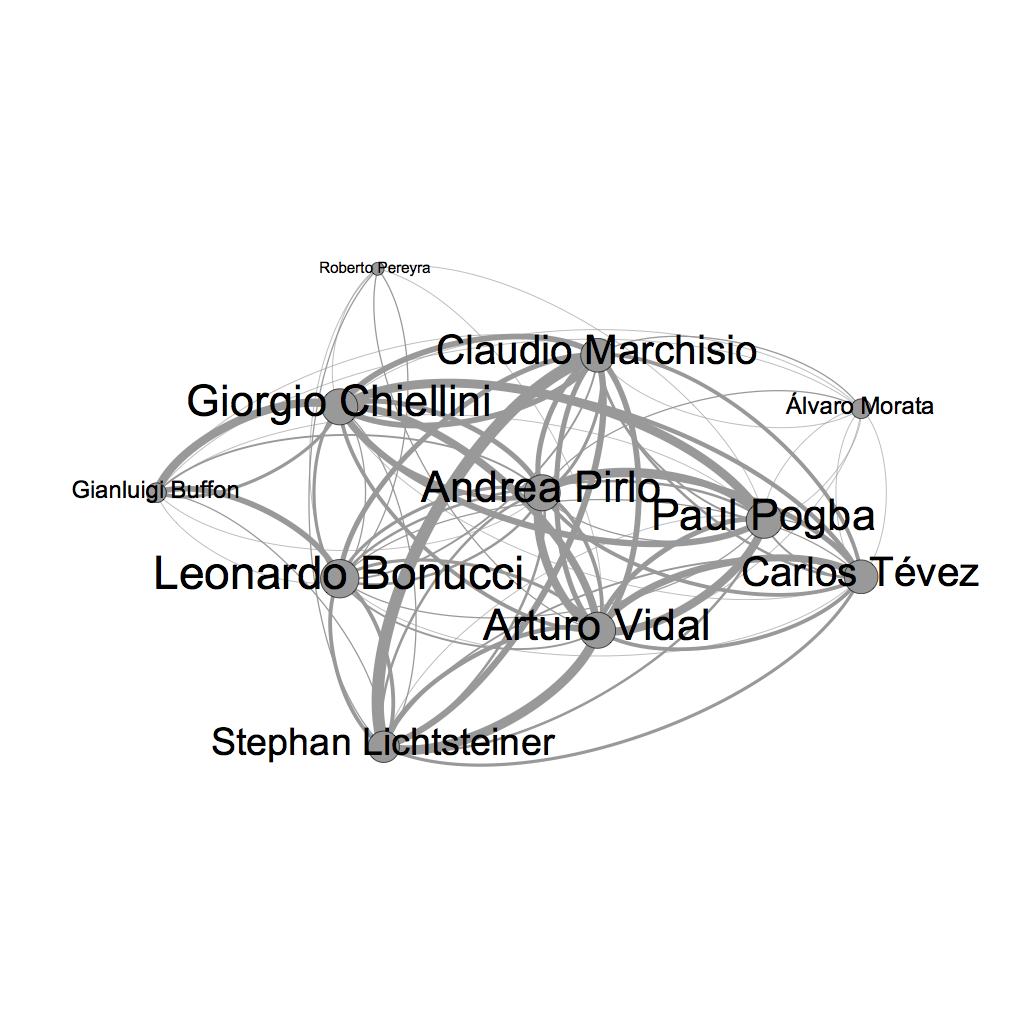
\includegraphics[scale=0.20]{2014372-Juventus-actual.png}
\label{fig:Juventus-group}
\end{figure}

\end{document}


